% Research paper - IEEE conference format (IEEEtran).
% Build: tectonic paper.tex   (or upload this folder to Overleaf)
% Every number comes from reports/ (see docs/PROJECT_REPORT.md, section 10).
\documentclass[conference]{IEEEtran}
\usepackage[T1]{fontenc}
\usepackage{cite}
\usepackage{amsmath}
\usepackage{newtxtext,newtxmath}  % Times, as in IEEE publications (provides amssymb symbols)
\usepackage{graphicx}
\usepackage{booktabs}
\usepackage{multirow}
\usepackage{xcolor}
\usepackage{tikz}
\usetikzlibrary{arrows.meta,positioning,fit}
\usepackage{url}
\usepackage[hidelinks]{hyperref}

\newcommand{\todo}[1]{\textcolor{red}{[#1]}}

\begin{document}

\title{Human-in-the-Loop Network Intrusion Detection with a Hybrid CNN-LSTM, Uncertainty-Aware Routing and Controlled Retraining}

\author{
\IEEEauthorblockN{Jai Chavan, Jeet Mane}
\IEEEauthorblockA{Department of Computer Engineering\\
Vidyalankar Institute of Technology, Mumbai, India\\
jai.chavan@vit.edu.in, jeet.mane@vit.edu.in}
\and
\IEEEauthorblockN{Dr. Kavita Shirsat}
\IEEEauthorblockA{Department of Computer Engineering\\
Vidyalankar Institute of Technology, Mumbai, India}
}

\maketitle

\begin{abstract}
Benchmark scores of learning-based intrusion detectors say little about what happens once live
traffic drifts away from what the detector was trained on. This paper describes a working
prototype built around that gap. Each network flow is first labelled by a convolutional-recurrent
(CNN-LSTM) classifier. A routing stage then decides whether the verdict can be acted on directly
or must be checked by a security analyst; it combines a temperature-scaled entropy score, a
Mahalanobis distance measured on the classifier's 128-dimensional embedding, and the vote spread
and agreement of a Random Forest acting as a second opinion. Analyst verdicts, with their stated
reasons and evidence, are kept in a searchable incident store, and they influence the model only
after an administrator has verified them and a retrained candidate has cleared thresholds declared
before training began. We evaluate the prototype on the corrected release of CIC-IDS2017, after
removing identifier columns and collapsing 385,106 duplicated flows before the data were split.
On 257,222 untouched test flows the deployed configuration forwards 1.48\% of traffic for review;
that queue holds 98.9\% of the classifier's mistakes, and the traffic handled without a human is
labelled with 99.999\% accuracy, with two attack flows dismissed and no benign flow escalated.
Withholding one attack family at a time shows that the classifier's own confidence collapses on
novel attacks (up to 97\% silently dismissed), whereas the combined router keeps such losses at
or below 10.2\% for five of the six withheld families. Brute-force SSH logins escaped every
configuration we tested. Finally, an extract-transform-load (ETL) job copies all 1,714,812
cleaned flows and the platform's own alerts and analyst decisions into a separate dimensional
data warehouse that supports online analytical processing (OLAP) without touching the detector.
\end{abstract}

\begin{IEEEkeywords}
intrusion detection, human-in-the-loop, uncertainty estimation, CNN-LSTM, out-of-distribution detection, CIC-IDS2017, selective classification, data warehouse, OLAP
\end{IEEEkeywords}

%=====================================================================
\section{Introduction}
Our starting point was a simple observation from our own first experiments: a Random Forest
trained in a few minutes already scored 99.97\% on a random split of CIC-IDS2017. If a quick
baseline can reach that figure, accuracy on such a split cannot be what separates a usable
detector from an unusable one. Three things weaken numbers of this kind. Flow datasets carry
mislabelled and repeated records that leak between training and test partitions
\cite{engelen2021troubleshooting,liu2022error}. Columns that identify hosts or sessions let a model
memorise rather than learn \cite{arp2022dos}. Above all, a deployed detector will sooner or later
receive an attack family absent from its training data, and a softmax output gives no reliable
signal when that happens \cite{sommer2010outside,hendrycks2017baseline}.

Our design follows an uncertainty-aware adaptive IDS proposed in \cite{refpaper2025}, which pairs
a CNN-LSTM with cWGAN-GP augmentation and analyst feedback and reports 98\% binary accuracy,
96.6\% detection rate, 92.1\% precision and 94.3\% F1. We rebuilt its classifier and turned the
idea into a complete application. Rather than asking how accurate the classifier is, we ask a
more operational question: for which flows may the classifier act alone, and which ones must a
person look at before anything is closed?

The paper makes three contributions.
\begin{enumerate}
\item We compare the CNN-LSTM with Random Forest and LightGBM on the corrected CIC-IDS2017 data
under strict leakage control (shortcut columns removed, duplicates collapsed before splitting,
three seeds), together with ablations that remove the LSTM or add synthetic samples.
\item Using withheld attack families and a split by capture day, we show that the network's own
uncertainty overlooks most novel attacks, and we propose a combined routing rule (entropy,
embedding distance, and a tree-ensemble second opinion) that sends most of them to an analyst.
\item We implement the full loop as software: traffic replay, an analyst console that captures
the reason behind each verdict, an incident store with similarity search, and retraining that is
gated by thresholds fixed in advance, administrator approval, live deployment and rollback.
Alongside it, a dimensional data warehouse filled by full and incremental ETL lets the traffic
history, alerts and analyst decisions be analysed with OLAP operations.
\end{enumerate}

%=====================================================================
\section{Related Work}
Our system draws on four strands of earlier work: the benchmark data and its known defects,
classifiers for tabular flow records, ways of estimating when a classifier should not be
trusted, and generative oversampling. Rather than restate each source, Table~\ref{tab:related}
lists what we took from it and where our system departs from it.

\begin{table*}[t]
\caption{Prior work used in this system}
\label{tab:related}
\centering
\footnotesize
\begin{tabular}{p{2.6cm}p{6.2cm}p{7.6cm}}
\toprule
Source & Idea relevant to us & How this project uses or extends it \\
\midrule
\cite{sharafaldin2018toward} & Five-day labelled flow capture (CIC-IDS2017) & Our only training and test source \\
\cite{engelen2021troubleshooting,liu2022error} & Flow and label errors found; corrected release published & We use the corrected files and add our own de-duplication before splitting \\
\cite{arp2022dos} & Leakage, shortcuts and weak baselines distort security ML & Identifier columns and destination port dropped; tree baselines on identical inputs \\
\cite{sommer2010outside} & Real networks are open-world; unseen activity is the norm & Motivates withholding whole attack families during evaluation \\
\cite{refpaper2025} & CNN-LSTM, cWGAN-GP and analyst feedback for adaptive IDS & Classifier rebuilt; feedback loop made controlled, verified and reversible \\
\cite{hochreiter1997lstm} & Gated recurrent memory & Recurrent layer over convolutional feature maps \\
\cite{breiman2001random,ke2017lightgbm} & Bagged and boosted tree ensembles & Baselines; the Random Forest also serves as second opinion \\
\cite{guo2017calibration} & One temperature parameter rescales logits & Fitted on half of the validation data \\
\cite{hendrycks2017baseline} & Softmax confidence flags many errors & Entropy score used as one routing signal \\
\cite{lee2018simple} & Distance to class centres in feature space flags unfamiliar inputs & Applied to the LSTM embedding \\
\cite{lakshminarayanan2017simple} & Independent models disagree on unfamiliar inputs & Disagreement between CNN-LSTM and Random Forest triggers review \\
\cite{geifman2017selective} & Trade abstention rate against error on accepted inputs & Referral rate vs.\ error on auto-handled flows \\
\cite{mirza2014conditional,gulrajani2017improved} & Class-conditional GAN with gradient penalty & Minority oversampling ablation \\
\bottomrule
\end{tabular}
\end{table*}

%=====================================================================
\section{Dataset and Preprocessing}
All experiments use the corrected CIC-IDS2017 files \cite{engelen2021troubleshooting,liu2022error},
one file per capture day from Monday to Friday. Together they hold 2,099,976 flow records, 91
columns and 27 distinct label strings. Our inspection script found no empty cells and only five
records with infinite byte- or packet-rate values. No two rows were identical as stored, yet once
the identifier columns were set aside, one row in eight (12.5\%) turned out to be a repeat.

\textit{Columns removed.} Flow ID, both IP addresses, the source port, the timestamp and the row
counter describe \emph{who} talked, not \emph{how}, so the model never sees them. The corrected
release adds an ``Attempted Category'' column that is only filled for attack rows; it would hand
the answer to the model and is discarded as well. We also leave out the destination port: in this
capture, port 21 is almost synonymous with FTP-Patator, which a model could exploit without
learning anything about the attack itself.

\textit{Label groups.} Every ``Attempted'' variant (an attack that did not succeed) is folded into
its parent attack. The \textit{Infiltration--Portscan} label is folded into \textit{Portscan},
since the two are indistinguishable in feature space, and brute-force, XSS and SQL-injection web
attacks form one ``Web Attack'' class. The result is 13 classes. Heartbleed (11 records) and
Infiltration (81 records) are kept but flagged: their per-class scores rest on a handful of test
flows, so we also report a ``reliable'' macro-F1 computed without them.

\textit{Removing repeats before the split.} Rows that agree on every input feature and on the
label are reduced to one copy, which removes 385,106 rows; a further 58 rows whose identical
features carry two different labels are dropped because no classifier could separate them.
Excluding the destination port exposed how repetitive the scan traffic is: Portscan shrank from
230,833 to 7,695 distinct flows. The 1,714,812 remaining flows are divided 70/15/15 with class
stratification (Table~\ref{tab:classes}), and hashing every feature vector confirms that no flow
occurs in more than one partition.

\textit{Feature transform.} Every statistic below is estimated on the training partition alone.
Infinite and missing values are replaced by the training median. Because byte and duration
counts span many orders of magnitude, each value is passed through $\mathrm{sign}(x)\log(1+|x|)$.
One column that never varies and 17 columns that almost duplicate another ($|\rho|>0.99$) are
dropped, leaving 64 inputs, which are then standardised. The fitted transform travels with every
saved model together with the column order and class list, so the web application applies
exactly the processing used in training.

\begin{table}[t]
\caption{Flows per class after mapping and de-duplication}
\label{tab:classes}
\centering
\footnotesize
\begin{tabular}{lrrr}
\toprule
Class & Train & Validation & Test \\
\midrule
BENIGN & 996,410 & 213,517 & 213,516 \\
DoS Hulk & 111,333 & 23,857 & 23,858 \\
DDoS & 66,601 & 14,272 & 14,271 \\
Portscan & 5,386 & 1,154 & 1,155 \\
DoS GoldenEye & 5,353 & 1,147 & 1,147 \\
DoS Slowloris & 3,992 & 855 & 856 \\
DoS Slowhttptest & 3,576 & 766 & 766 \\
FTP-Patator & 2,789 & 597 & 598 \\
SSH-Patator & 2,092 & 448 & 448 \\
Web Attack & 1,439 & 309 & 308 \\
Botnet & 1,343 & 288 & 288 \\
Infiltration$^\dagger$ & 46 & 10 & 10 \\
Heartbleed$^\dagger$ & 8 & 2 & 1 \\
\midrule
Total & 1,200,368 & 257,222 & 257,222 \\
\bottomrule
\multicolumn{4}{l}{$^\dagger$Too few samples for reliable per-class metrics.}
\end{tabular}
\end{table}

%=====================================================================
\section{Methodology}

\begin{figure*}[t]
\centering
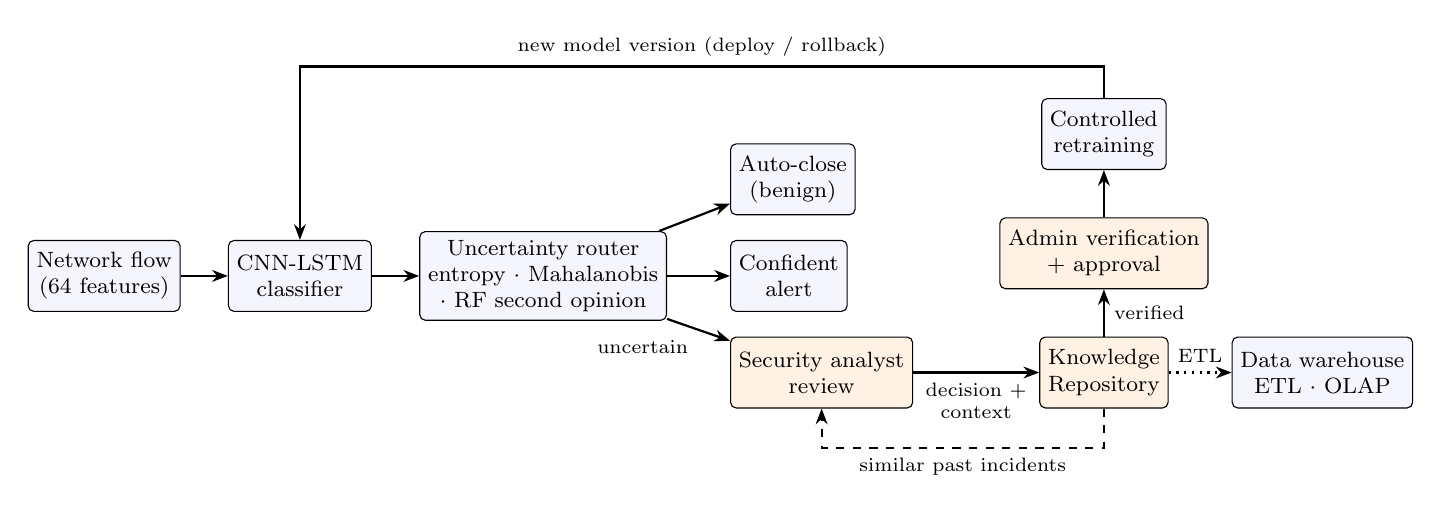
\begin{tikzpicture}[
  box/.style={draw, rounded corners=2pt, align=center, font=\footnotesize, minimum height=9mm, inner sep=3pt, fill=blue!4},
  hum/.style={box, fill=orange!10},
  arr/.style={-{Stealth[length=2mm]}, thick},
  lab/.style={font=\scriptsize, align=center}]
\node[box] (flow) {Network flow\\(64 features)};
\node[box, right=6mm of flow] (cnn) {CNN-LSTM\\classifier};
\node[box, right=6mm of cnn] (unc) {Uncertainty router\\entropy $\cdot$ Mahalanobis\\$\cdot$ RF second opinion};
\node[box, above right=2mm and 8mm of unc] (benign) {Auto-close\\(benign)};
\node[box, right=8mm of unc] (alert) {Confident\\alert};
\node[hum, below right=2mm and 8mm of unc] (analyst) {Security analyst\\review};
\node[hum, right=16mm of analyst] (kr) {Knowledge\\Repository};
\node[hum, above=6mm of kr] (admin) {Admin verification\\+ approval};
\node[box, above=6mm of admin] (retrain) {Controlled\\retraining};
\node[box, right=8mm of kr] (dw) {Data warehouse\\ETL $\cdot$ OLAP};
\draw[arr] (flow) -- (cnn);
\draw[arr] (cnn) -- (unc);
\draw[arr] (unc) -- (benign);
\draw[arr] (unc) -- (alert);
\draw[arr] (unc) -- node[lab, below left]{uncertain} (analyst);
\draw[arr] (analyst) -- node[lab, below]{decision +\\context} (kr);
\draw[arr] (kr) -- node[lab, right]{verified} (admin);
\draw[arr] (admin) -- (retrain);
\draw[arr] (retrain.north) |- ++(0,4mm) -| node[lab, above, pos=0.25]{new model version (deploy / rollback)} (cnn.north);
\draw[arr, dashed] (kr.south) |- ++(0,-5mm) -| node[lab, below, pos=0.25]{similar past incidents} (analyst.south);
\draw[arr, dotted] (kr) -- node[lab, above]{ETL} (dw);
\end{tikzpicture}
\caption{System overview. Only uncertain flows reach the analyst; verified analyst decisions
improve the model only through administrator-approved retraining. A separate data warehouse,
filled by ETL, is used for analysis only.}
\label{fig:system}
\end{figure*}

\subsection{Classifier}
The layer sequence is taken from Table 5 of \cite{refpaper2025}, with 64 inputs instead of 46.
The standardised feature vector is read as a single-channel signal of length 64 and passes through
a 64-filter convolution (kernel 5, ReLU), max-pooling by two, a 128-filter convolution (kernel 3,
ReLU), an LSTM with 128 units, dropout of 0.3 and a 13-way linear output. We keep the last LSTM
state $\mathbf{z}\in\mathbb{R}^{128}$ as an embedding of the flow, since later stages measure
distances in that space. Training uses ordinary cross-entropy with AdamW (learning rate
$10^{-3}$, batches of 1,024, cosine decay), up to 20 epochs, and keeps the epoch with the best
validation macro-F1. We avoided class-weighted loss because it shifts the predicted probabilities
that the routing stage relies on. Our first runs, however, never once predicted Heartbleed or
Infiltration, which held validation macro-F1 near 0.85; copying the rows of any class with fewer
than 1,000 training examples until it reaches that count (training partition only) fixed this.

\subsection{Baselines and ablations}
A 100-tree Random Forest and a LightGBM model receive exactly the same 64 transformed inputs.
LightGBM stops early on validation loss; in our first attempt it diverged after 12 boosting
rounds, which a cap on leaf output values resolved. Three ablations probe the design: replacing
the LSTM with global average pooling, adding GAN-generated minority samples, and skipping
temperature scaling.

\subsection{Minority augmentation}
For the augmentation ablation we train a class-conditional Wasserstein GAN with gradient penalty
\cite{mirza2014conditional,gulrajani2017improved}. Generator and critic each have two hidden layers
of 256 units; the penalty weight is 10 and the critic is updated five times per generator update.
Only classes with between 100 and 5,000 training rows are topped up, to 5,000 rows each. A
generated row is accepted only when the baseline Random Forest assigns it to the class it was
generated for. The reference design seeds its generator with a VAE; ours starts from Gaussian
noise.

\subsection{Calibration and uncertainty signals}
We cut the validation partition into two stratified halves. The first (``calibration'') half is
used to fit everything in this subsection; the second (``evaluation'') half is reserved for
judging the result. A single temperature $T$ \cite{guo2017calibration} rescales the logits, after
which every flow receives two scores:
\begin{equation}
H(\mathbf{x}) = -\frac{1}{\log K}\sum_{k=1}^{K} p_k \log p_k, \quad
\mathbf{p} = \mathrm{softmax}(\mathbf{f}(\mathbf{x})/T),
\end{equation}
an entropy over the $K=13$ classes scaled to lie between 0 and 1, and the squared Mahalanobis
distance from the flow's embedding to the nearest class centre \cite{lee2018simple}
\begin{equation}
D(\mathbf{x}) = \min_{c} (\mathbf{z}-\boldsymbol{\mu}_c)^\top \boldsymbol{\Sigma}^{-1} (\mathbf{z}-\boldsymbol{\mu}_c),
\end{equation}
where the centres $\boldsymbol{\mu}_c$ and one pooled covariance $\boldsymbol{\Sigma}$ (with a
small ridge added for stability) come from training-set embeddings. Entropy captures hesitation
between known classes; the distance captures flows that resemble none of them. Each score gets a
cut-off read from the calibration half: $\tau_H$ is the value exceeded by its most uncertain 1\%
of flows, and $\tau_D$ the value exceeded by its most distant 0.5\%.

\subsection{Hybrid routing}
A flow is \emph{uncertain} if
\begin{equation}
H>\tau_H \;\lor\; D>\tau_D \;\lor\; u_{\mathrm{RF}}>\tau_{\mathrm{RF}} \;\lor\; \hat{y}_{\mathrm{RF}}\neq\hat{y},
\end{equation}
and each flow receives one of three decisions:
\begin{equation}
\text{decision}(\mathbf{x}) =
\begin{cases}
\text{review} & \text{if uncertain},\\
\text{auto-alert} & \text{else if } \hat{y}\neq\text{BENIGN},\\
\text{auto-benign} & \text{otherwise,}
\end{cases}
\end{equation}
Here $\hat{y}$ denotes the CNN-LSTM's predicted class and $\hat{y}_{\mathrm{RF}}$ the Random
Forest's. The forest's own doubt is $u_{\mathrm{RF}} = 1-\max_k p^{\mathrm{RF}}_k$, i.e.\ the
share of trees that did not vote for the winning class, and $\tau_{\mathrm{RF}}$ flags its most
doubtful 0.5\% of calibration flows. In words: a flow is closed or escalated automatically only
when the network is decisive, the flow lies close to familiar traffic, and an independently
trained forest is both confident and in agreement. We introduced the two forest terms only after
the withheld-family experiment (Section~\ref{sec:loao}) exposed how often the network alone
dismissed novel attacks. That experiment therefore cannot count as independent evidence for the
combined rule; the test partition, opened once and only after the rule was frozen, can.

\subsection{Human-in-the-loop platform}
Fig.~\ref{fig:system} shows how the parts connect. The back end is a FastAPI service backed by
SQLite; the front end is a React application with four areas: a public About page, an analyst
console, an administration console and a data-warehouse view (Section~\ref{sec:dw}).
\begin{itemize}
\item \textit{Replay.} To imitate live traffic, a background worker feeds the untouched test
partition to the active model in configurable batches. Each record's true label is stored beside
it purely so the administrator can measure live accuracy; it never enters the model and is never
returned to analyst screens, a property checked by an automated test.
\item \textit{Analyst console.} A referred flow opens on one screen showing its addresses, ports
and time, the three most likely classes, the forest's opinion, both uncertainty scores drawn
against their cut-offs, the six features furthest from typical training values, and the most
similar earlier incidents. The analyst answers with a verdict (malicious, benign or unsure), a
class, and free-text reason, context and evidence, plus a confidence level and tags.
\item \textit{Incident store.} Every answer is saved as a searchable incident. Similarity between
incidents is the cosine of their CNN-LSTM embeddings; because a retrained network maps flows to a
different space, the stored embeddings are recomputed whenever the active model changes.
\item \textit{Gated retraining.} Feedback becomes training data only after an administrator marks
it as verified. The verified items are split 70/30. The active network is fine-tuned on the 70\%
together with 200,000 rows drawn from the original training partition, so that it does not forget
older attack families, and is then recalibrated. Old and new models are compared on two fixed
yardsticks: the evaluation half of the validation partition and the 30\% of feedback held back.
The pass mark is written in a configuration file and copied into each job when the job is
created: reliable macro-F1 may fall by no more than 0.5 points, the false-positive rate may rise
by no more than 0.05 points, and accuracy on the held-back feedback may not fall. Even a passing
candidate goes live only after an administrator approves it; deploying or rolling back replaces
the model in memory while the service keeps running, and each step is recorded in an audit log.
\end{itemize}

\subsection{Analytical data warehouse}\label{sec:dw}
The platform's database is an operational (OLTP) store: normalised tables that receive many small
writes. Questions over the whole traffic history, such as how much denial-of-service traffic
reached web services in each hour, are better answered from a separate, read-mostly copy organised
for analysis \cite{chaudhuri1997overview,kimball2013toolkit}. We therefore added a data warehouse
in its own SQLite file. It is purely descriptive: it never feeds training, tuning, prediction or the
analyst's decision.
\begin{itemize}
\item \textit{ETL.} \emph{Extract} reads the three cleaned partitions, the raw capture files
(for timestamps) and, read-only, the platform database. \emph{Transform} joins every flow to its
raw record on day and row identifier (all 1,714,812 matched), sets missing or negative measures to
zero, derives total packets and bytes, converts durations to milliseconds, generalises destination
ports to services and port ranges, and assigns surrogate keys. \emph{Load} builds the whole
warehouse in a staging file and swaps it in at once (full load, 25\,s). Later runs use
incremental extraction: only alerts whose identifier exceeds a stored watermark are appended
(0.3\,s when nothing is new), and a reset of the platform database is detected and handled.
\item \textit{Schemas.} The central fact table holds one row per flow, with keys to five
dimensions (time to the minute, attack class with category and severity, service, protocol, and
data partition) and the packet, byte and duration measures, forming a star schema. A snowflake
variant normalises the attack and time dimensions into category and date sub-dimensions. A fact
constellation joins an alert fact table (model output) and a factless review table (analyst
decisions) through shared, conformed time, attack and model dimensions.
\item \textit{OLAP.} A cube view offers roll-up, drill-down, slice, dice and pivot over these
hierarchies. Each operation is translated into a parameterised SQL query, which is shown to the
user. Queries that need only time (down to the hour) and attack class are answered automatically
from a pre-summed hourly aggregate table of 82 rows instead of the full fact table.
\end{itemize}

%=====================================================================
\section{Experimental Setup}
Models are fitted on the training partition, and every choice of settings or design was made by
looking at validation results only. We opened the test partition a single time, once the routing
rule and all settings were frozen. Each model was trained with three seeds (42, 7 and 2025), and
tables give the mean and standard deviation across them; the deployed application uses the seed-42
network and forest. ``Accuracy'' counts a prediction as correct only if the exact one of 13
classes is right. Precision, detection rate (recall), F1, false-positive rate (FPR) and
false-negative rate instead pool all attacks into one positive class, as the reference work does.
Everything ran on a laptop with an Intel Core i5-1240P, 7.7\,GB of RAM and an NVIDIA RTX 2050
(4\,GB), using PyTorch \cite{paszke2019pytorch} and scikit-learn \cite{pedregosa2011scikit}.

\textit{Generalisation tests.} Two further experiments use only training and validation rows.
(i) \emph{Withheld family:} for each of six attacks we delete every row of that attack from the
data used for training and calibration, refit the whole chain with one seed (eight CNN-LSTM epochs,
temperature, cut-offs and forest), and then record what the router does with that attack's flows.
(ii) \emph{Split by day:} we fit on Monday to Wednesday traffic and evaluate on Thursday and
Friday, whose attack types never occur earlier in the week.

%=====================================================================
\section{Results}

\subsection{Classification on the held-out test set}
Table~\ref{tab:main} sets every model beside the figures published for the reference design. All
five of our models, the rebuilt CNN-LSTM included, score above those figures on every binary
metric. We do not read this as an improvement on that work: the data release, the duplicate
handling and the removed columns all differ, and such choices alone are known to move results a
great deal \cite{engelen2021troubleshooting,arp2022dos}. Within our own comparison the tree
ensembles come out ahead. The Random Forest reaches 99.23\% reliable macro-F1 against the
CNN-LSTM's 98.09\%, and raises roughly a third as many false alarms (FPR 0.020\% vs.\ 0.059\%).

\begin{table*}[t]
\caption{Held-out test set (257,222 flows), mean $\pm$ standard deviation over three seeds (\%)}
\label{tab:main}
\centering
\footnotesize
\begin{tabular}{lcccccc}
\toprule
Metric & Reported \cite{refpaper2025} & Random Forest & LightGBM & CNN-LSTM & CNN-LSTM + aug. & CNN (no LSTM) \\
\midrule
Accuracy & 98.0$^\ast$ & \textbf{99.97} $\pm$ 0.00 & 99.96 $\pm$ 0.00 & 99.89 $\pm$ 0.07 & 99.92 $\pm$ 0.02 & 99.80 $\pm$ 0.02 \\
Detection rate & 96.6 & \textbf{99.92} $\pm$ 0.00 & 99.91 $\pm$ 0.01 & 99.75 $\pm$ 0.24 & 99.86 $\pm$ 0.05 & 99.23 $\pm$ 0.10 \\
Precision & 92.1 & \textbf{99.90} $\pm$ 0.00 & 99.84 $\pm$ 0.01 & 99.71 $\pm$ 0.07 & 99.74 $\pm$ 0.03 & 99.70 $\pm$ 0.01 \\
F1 & 94.3 & \textbf{99.91} $\pm$ 0.00 & 99.88 $\pm$ 0.01 & 99.73 $\pm$ 0.16 & 99.80 $\pm$ 0.04 & 99.46 $\pm$ 0.05 \\
Macro-F1 (13 classes) & -- & \textbf{99.07} $\pm$ 0.22 & 98.32 $\pm$ 0.04 & 96.71 $\pm$ 3.06 & 97.46 $\pm$ 1.36 & 94.12 $\pm$ 1.42 \\
Macro-F1 (reliable) & -- & \textbf{99.23} $\pm$ 0.02 & 99.03 $\pm$ 0.05 & 98.09 $\pm$ 0.99 & 98.47 $\pm$ 0.25 & 96.39 $\pm$ 0.32 \\
FPR & -- & \textbf{0.020} $\pm$ 0.000 & 0.033 $\pm$ 0.003 & 0.059 $\pm$ 0.015 & 0.054 $\pm$ 0.005 & 0.062 $\pm$ 0.002 \\
\bottomrule
\multicolumn{7}{l}{$^\ast$Binary accuracy in \cite{refpaper2025}; ours is 13-class accuracy. ``Reliable'' excludes Heartbleed and Infiltration.}
\end{tabular}
\end{table*}

\begin{table}[t]
\caption{Per-class recall on the test set (\%, mean over three seeds)}
\label{tab:perclass}
\centering
\footnotesize
\begin{tabular}{lccc}
\toprule
Class & RF & LightGBM & CNN-LSTM \\
\midrule
BENIGN & 99.98 & 99.97 & 99.94 \\
DoS Hulk & 100.00 & 99.99 & 99.90 \\
DDoS & 100.00 & 100.00 & 99.99 \\
Portscan & 99.65 & 99.65 & 96.65 \\
DoS GoldenEye & 100.00 & 99.91 & 98.23 \\
DoS Slowloris & 100.00 & 100.00 & 99.10 \\
DoS Slowhttptest & 98.87 & 99.09 & 98.96 \\
FTP-Patator & 100.00 & 100.00 & 99.78 \\
SSH-Patator & 99.70 & 99.70 & 99.48 \\
Web Attack & 97.94 & 98.38 & 96.54 \\
Botnet & 94.79 & 92.01 & 89.35 \\
Infiltration$^\dagger$ & 93.33 & 80.00 & 93.33 \\
Heartbleed$^\dagger$ & 100.00 & 100.00 & 100.00 \\
\bottomrule
\multicolumn{4}{l}{$^\dagger$10 and 1 test flows respectively.}
\end{tabular}
\end{table}

Looking class by class (Table~\ref{tab:perclass}), the network's shortfall is concentrated in
three classes: Portscan, Botnet and Web Attack. Botnet is the weakest of the reliable classes for
all three models, with recall between 89\% and 95\%.

\subsection{Ablations}
Taking the LSTM out costs 1.7 points of reliable macro-F1 and drops Portscan recall from 96.7\% to
88.8\%, so the recurrent layer does earn its place. Adding generated minority samples lifts mean
reliable macro-F1 by 0.4 points and makes the three seeds agree more closely (standard deviation
falls from 0.99 to 0.25); the gain is, however, smaller than the spread between seeds. A simple
check explains why the effect is modest: a classifier asked to tell real from generated rows
separates them perfectly (AUC 1.0) for all six topped-up classes, because real flow features are
integer counts whereas the generator emits smooth real values. Temperature scaling settled on
$T=1.01$, meaning the network's confidence was already in line with its accuracy (calibration
error 0.023\% before and 0.022\% after); dropping this step changes nothing measurable here.

\subsection{Routing on the test set}
Table~\ref{tab:routing} summarises the configuration that runs in the application. One flow in
roughly 68 (1.48\%) is put in front of an analyst, and that small queue contains 98.9\% of all the
mistakes the network makes. On the remaining 98.5\% of traffic, which nobody reviews, the labels
are correct 99.999\% of the time. Out of 43,706 attack flows, two were closed as benign, and not a
single benign flow was escalated as a confident alert. Against routing with the network's own two
scores, the forest adds 0.15 percentage points of review work and cuts dismissed attacks from seven
to two. The review load falls where the classifier is least reliable: every Infiltration flow,
99.7\% of Web Attack, 75\% of DoS Slowhttptest, 63\% of Botnet and 38\% of Portscan flows reach an
analyst, compared with under 1\% for BENIGN, DDoS and DoS Hulk.

\begin{table}[t]
\caption{Deployed routing on the test set}
\label{tab:routing}
\centering
\footnotesize
\begin{tabular}{lcc}
\toprule
 & Hybrid & CNN-LSTM \\
 & (deployed) & signals only \\
\midrule
Referred to analyst & 1.48\% & 1.33\% \\
Accuracy, auto-handled & \textbf{99.999\%} & 99.997\% \\
Errors caught by review & \textbf{98.9\%} & 96.0\% \\
Attacks auto-closed & \textbf{2} & 7 \\
Benign auto-alerted & 0 & 0 \\
\bottomrule
\end{tabular}
\end{table}

\subsection{Unseen attacks: leave-one-attack-out}
\label{sec:loao}
For each withheld family, Fig.~\ref{fig:loao} plots the fraction of its flows that the router
closed as benign, i.e.\ the attacks nobody would ever have seen. Our first pass of this experiment
is what changed the design: relying on its own two scores, the network dismissed 80.5\% of the
unseen Portscan flows and 32.9\% of the unseen Botnet flows, while a Random Forest that only looked
at how its trees split their votes dismissed 5.3\% and 10.8\%. The network also behaved
inconsistently from one training run to the next: unseen web attacks were dismissed 13.1\% of the
time in the first pass and 97.0\% in the pass plotted here. With the combined rule, dismissals
were lowest for five families out of six and never above 10.2\% for those five; the price is that
about 1.4\% of ordinary traffic is reviewed, where the forest alone needs 0.55\%. SSH brute force
got past every variant: taken one at a time, its login attempts look exactly like genuine SSH
sessions.

\begin{figure}[t]
\centering
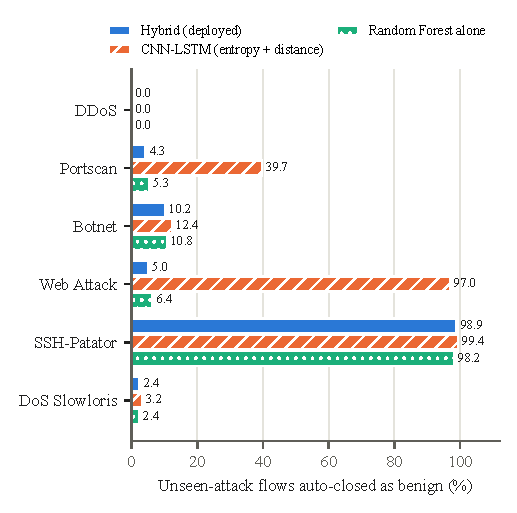
\includegraphics[width=\columnwidth]{figs/loao_missed.pdf}
\caption{Leave-one-attack-out: share of the held-out attack's flows auto-closed as benign
(lower is better). Each group retrains the full pipeline without that attack.}
\label{fig:loao}
\end{figure}

\subsection{Unseen days}
When the models see only Monday to Wednesday and are tested on Thursday and Friday, the combined
rule closes 1.38\% of attack flows as benign. Using the network's entropy alone, that figure is
35.28\%; adding the embedding distance brings it down to 16.46\%, so the distance score does real
work, but only the forest's opinion brings losses down to the level of the forest by itself
(1.45\%). Ordinary traffic sent for review rises to 0.76\%, against 0.50\% for the forest alone.
Broken down by class (Fig.~\ref{fig:day}), Botnet is the clear weak spot, with 37.7\% of its flows
closed unseen.

\begin{figure}[t]
\centering
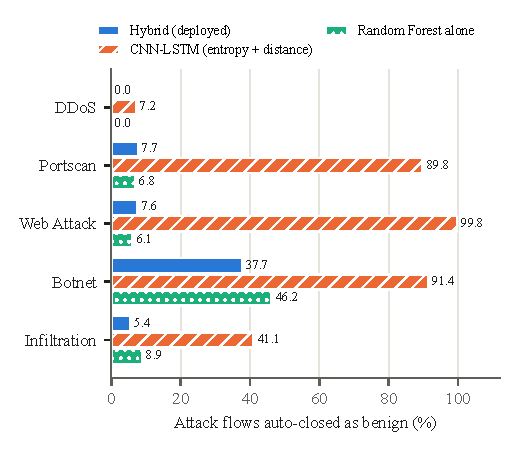
\includegraphics[width=\columnwidth]{figs/day_missed.pdf}
\caption{Day-based split (train Monday--Wednesday, evaluate Thursday--Friday): share of each
unseen attack class auto-closed as benign.}
\label{fig:day}
\end{figure}

\subsection{System behaviour}
While replaying traffic, the service needs about 0.55\,ms of CPU time per flow, forest included.
One automated test walks through a whole working session: traffic is replayed, an analyst records
verdicts, similar incidents are retrieved, an administrator verifies feedback, a candidate is
retrained and checked, then approved, deployed and rolled back, and every step must appear in the
audit log. The same test confirms that no analyst-facing response ever contains a true label.

For the warehouse, a question such as flows per attack class per day takes about 2.0\,s on the
1.7-million-row fact table but about 0.1\,ms on the hourly aggregate, with an identical answer.
The same question by category runs in about 2.0\,s on the star schema and 2.3\,s on the
snowflake variant, whose extra joins cost time but remove repeated values. Automated tests check a
full and an incremental load, the detection of a platform reset, and that OLAP results built from
the aggregate equal those built from the fact table.

%=====================================================================
\section{Discussion}
\textit{What the numbers do and do not show.} With leakage removed, every model we trained passes
99.7\% binary F1 on a random split, and the forest edges out the network. On such a split the
contest is effectively over before it starts; the differences that matter for an operator only
appear when the traffic contains something the model has not met before.

\textit{Confidence is not safety.} The network's own scores let up to 97\% of a novel attack
through, and how badly it failed changed from run to run. The single change that helped most was
to pair it with a model built on entirely different principles and to send their disagreements to
a person. This is in line with earlier evidence that several independent models express doubt
more reliably than one network does \cite{lakshminarayanan2017simple}.

\textit{Caveats.} The combined rule was chosen after we had seen the withheld-family results, so
those results flatter it. The test partition was used only once, but it contains no attack type
that the models had not met in training. Each withheld family was run with a single seed. Our
comparison with the reference paper differs in data release and preprocessing. The two classes
with fewer than 100 records cannot be scored meaningfully. Finally, the analyst workflow was
exercised by the authors rather than by working security staff.

\textit{Limitations.} A model that judges one flow at a time cannot see attacks that only make
sense across many flows, such as SSH password guessing and part of the botnet traffic; features
summarising a host's activity over a time window would be needed. Retraining currently updates
the network but not the forest. The generator's samples are unrealistic, so generation that
respects integer-valued features, or the VAE seeding of the reference design, is worth trying.
Login and access control in the prototype are simulated.

%=====================================================================
\section{Conclusion}
This work set out to build an intrusion detector that knows when to hand a decision to a person.
Under careful leakage control, our CNN-LSTM comes close to strong tree baselines and scores above
the figures published for the reference design, yet its own sense of uncertainty breaks down on
attacks it has never met. Adding a Random Forest as a second opinion fixes most of that: only
1.48\% of traffic needs a human, that share contains 98.9\% of the network's errors, and most
flows from withheld attack families end up with an analyst instead of being closed silently.
Analyst knowledge flows back into the model only through verified, threshold-gated and
administrator-approved retraining that can be undone, and a separate data warehouse makes the
whole traffic and decision history available for OLAP analysis. Next steps are features that summarise many
flows per host, retraining the forest alongside the network, and testing on CSE-CIC-IDS2018 to see
how the system copes with a different network.

\section*{Acknowledgment}
The authors are grateful to Dr. Kavita Shirsat for the guidance, review and encouragement
throughout this project, and to the Department of Computer Engineering, Vidyalankar Institute of
Technology, Mumbai, for providing the laboratory facilities and computing resources used in this
work. We also thank the maintainers of the corrected CIC-IDS2017 dataset for making it publicly
available.

%=====================================================================
\begin{thebibliography}{99}

\bibitem{refpaper2025}
C.~M. de~Nascimento and J.~Hou, ``Uncertainty-aware adaptive intrusion detection using hybrid CNN-LSTM with cWGAN-GP augmentation and human-in-the-loop feedback,'' \textit{Safety}, vol.~11, no.~4, Art.~no.~120, Dec. 2025, doi: 10.3390/safety11040120.

\bibitem{sharafaldin2018toward}
I.~Sharafaldin, A.~H. Lashkari, and A.~A. Ghorbani, ``Toward generating a new intrusion detection dataset and intrusion traffic characterization,'' in \textit{Proc. 4th Int. Conf. Information Systems Security and Privacy (ICISSP)}, 2018, pp. 108--116.

\bibitem{engelen2021troubleshooting}
G.~Engelen, V.~Rimmer, and W.~Joosen, ``Troubleshooting an intrusion detection dataset: the CICIDS2017 case study,'' in \textit{Proc. IEEE Security and Privacy Workshops (SPW)}, 2021, pp. 7--12.

\bibitem{liu2022error}
L.~Liu, G.~Engelen, T.~Lynar, D.~Essam, and W.~Joosen, ``Error prevalence in NIDS datasets: A case study on CIC-IDS-2017 and CSE-CIC-IDS-2018,'' in \textit{Proc. IEEE Conf. Communications and Network Security (CNS)}, 2022, pp. 254--262.

\bibitem{arp2022dos}
D.~Arp \textit{et al.}, ``Dos and don'ts of machine learning in computer security,'' in \textit{Proc. 31st USENIX Security Symposium}, 2022, pp. 3971--3988.

\bibitem{sommer2010outside}
R.~Sommer and V.~Paxson, ``Outside the closed world: On using machine learning for network intrusion detection,'' in \textit{Proc. IEEE Symposium on Security and Privacy}, 2010, pp. 305--316.

\bibitem{hochreiter1997lstm}
S.~Hochreiter and J.~Schmidhuber, ``Long short-term memory,'' \textit{Neural Computation}, vol.~9, no.~8, pp. 1735--1780, 1997.

\bibitem{breiman2001random}
L.~Breiman, ``Random forests,'' \textit{Machine Learning}, vol.~45, no.~1, pp. 5--32, 2001.

\bibitem{ke2017lightgbm}
G.~Ke \textit{et al.}, ``LightGBM: A highly efficient gradient boosting decision tree,'' in \textit{Advances in Neural Information Processing Systems (NeurIPS)}, 2017, pp. 3146--3154.

\bibitem{guo2017calibration}
C.~Guo, G.~Pleiss, Y.~Sun, and K.~Q. Weinberger, ``On calibration of modern neural networks,'' in \textit{Proc. 34th Int. Conf. Machine Learning (ICML)}, 2017, pp. 1321--1330.

\bibitem{hendrycks2017baseline}
D.~Hendrycks and K.~Gimpel, ``A baseline for detecting misclassified and out-of-distribution examples in neural networks,'' in \textit{Proc. Int. Conf. Learning Representations (ICLR)}, 2017.

\bibitem{lee2018simple}
K.~Lee, K.~Lee, H.~Lee, and J.~Shin, ``A simple unified framework for detecting out-of-distribution samples and adversarial attacks,'' in \textit{Advances in Neural Information Processing Systems (NeurIPS)}, 2018, pp. 7167--7177.

\bibitem{lakshminarayanan2017simple}
B.~Lakshminarayanan, A.~Pritzel, and C.~Blundell, ``Simple and scalable predictive uncertainty estimation using deep ensembles,'' in \textit{Advances in Neural Information Processing Systems (NeurIPS)}, 2017, pp. 6402--6413.

\bibitem{geifman2017selective}
Y.~Geifman and R.~El-Yaniv, ``Selective classification for deep neural networks,'' in \textit{Advances in Neural Information Processing Systems (NeurIPS)}, 2017, pp. 4878--4887.

\bibitem{mirza2014conditional}
M.~Mirza and S.~Osindero, ``Conditional generative adversarial nets,'' \textit{arXiv preprint arXiv:1411.1784}, 2014.

\bibitem{gulrajani2017improved}
I.~Gulrajani, F.~Ahmed, M.~Arjovsky, V.~Dumoulin, and A.~C. Courville, ``Improved training of Wasserstein GANs,'' in \textit{Advances in Neural Information Processing Systems (NeurIPS)}, 2017, pp. 5767--5777.

\bibitem{paszke2019pytorch}
A.~Paszke \textit{et al.}, ``PyTorch: An imperative style, high-performance deep learning library,'' in \textit{Advances in Neural Information Processing Systems (NeurIPS)}, 2019, pp. 8024--8035.

\bibitem{pedregosa2011scikit}
F.~Pedregosa \textit{et al.}, ``Scikit-learn: Machine learning in Python,'' \textit{Journal of Machine Learning Research}, vol.~12, pp. 2825--2830, 2011.

\bibitem{chaudhuri1997overview}
S.~Chaudhuri and U.~Dayal, ``An overview of data warehousing and OLAP technology,'' \textit{ACM SIGMOD Record}, vol.~26, no.~1, pp. 65--74, 1997.

\bibitem{kimball2013toolkit}
R.~Kimball and M.~Ross, \textit{The Data Warehouse Toolkit: The Definitive Guide to Dimensional Modeling}, 3rd~ed. Indianapolis, IN, USA: Wiley, 2013.

\end{thebibliography}

\end{document}
